% !TeX encoding = UTF-8
% !TeX spellcheck = fr_FR

%%%%%%%%%%%%%%%%%%%%%%%%%%%%%%%%%%%%%%%%%%%%%%%%%%%%%%
% Concours commun INP                                %
% https://www.concours-commun-inp.fr                 %
% CC BY-NC-SA, Novembre 2023                         %
% https://creativecommons.org/licenses/by-nc-sa/4.0/ %
%%%%%%%%%%%%%%%%%%%%%%%%%%%%%%%%%%%%%%%%%%%%%%%%%%%%%%

% Pour compiler : lualatex -shell-escape
\documentclass{ccinp}

\lfoot{\includegraphics[width=5em]{by-nc-sa.eu.png}}
\cfoot{\thepage}
\rfoot{28 octobre 2024}

% A décommenter pour enlever la correction
% \excludecomment{correction}

\begin{document}


\title{Sélection de sujets posés lors de la session 2024}
\date{}



\maketitle
\thispagestyle{fancy}

\section*{Exercices de type A}


\exocommand{Une relation d'équivalence (type A)}

On fixe $n\in \mathbb{N}^{\star}$. Soient  $\varphi : \llbracket 1,n\rrbracket \to \llbracket 1,n \rrbracket $ et $\psi : \llbracket 1,n\rrbracket \to  \llbracket 1,n\rrbracket$.
Soit $u$ et  $v$ deux éléments
de  $\llbracket 1,n \rrbracket$. On dit que  $u$ et  $v$ sont $(\varphi,\psi)$-équivalents s'il existe  $k\in \mathbb{N}$, un tuple $(w_0,w_1,\cdots , w_{k+1}) \in \llbracket 1,n \rrbracket^{k+2}$ avec $w_0=u, w_{k+1}= v$ et vérifiant : 
$$ \forall i \in \llbracket 0,k \rrbracket, \varphi(w_{i})=\varphi(w_{i+1}) \mbox { ou } \psi(w_{i})=\psi(w_{i+1}).$$
L'objectif est d'écrire un algorithme en pseudo-code permettant de calculer les différentes classes d'équivalence engendrées par cette relation. 

 \begin{enumerate}
     \item Justifier rapidement que "être $(\varphi,\psi)$-équivalent" est une relation d'équivalence sur l'ensemble $\llbracket 1,n \rrbracket$.
     \item Pour cette question, on considère les applications $\varphi$ et  $\psi$ définies par :
         \begin{equation*}
             \begin{array}{| c| l| l | l | l | l | l | l |  l | l | l |}
                 \hline  
                 i=  & 1 & 2 & 3 & 4 & 5 & 6 & 7 & 8 & 9 \\ 
                 \hline 
                 \varphi(i) =&   3 & 2 & 2 & 9 & 6 & 4 & 9 & 5 & 7 \\ 
                 \hline 
                 \psi(i) =&   5 & 1 & 3 & 4 & 5 & 1 & 7 & 7 & 4 \\ 
                 \hline 
             \end{array}
         \end{equation*}
         Calculer les différentes classes d'équivalence.
     \item On revient au cas au général. On définit le graphe $G =(S,A)$ par :
         $$ S = \llbracket 1, n \rrbracket , A = \{(x,y) \in S^2 | x\neq y \mbox{ et } (\varphi(x) = \varphi(y) \mbox{ ou } \psi(x) = \psi(y) ) \}.$$
         On fixe $x$ et  $y$ deux sommets différents de  $S$. Traduire sur le graphe $G$ le fait que les sommets $x$ et $y$ sont $(\varphi,\psi)$-équivalents et en déduire que le calcul des classes d'équivalence de  $G$ se traduit en un problème classique sur les graphes que l'on précisera. 
     \item Donner en pseudo-code un algorithme permettant de résoudre le problème correspondant
         sur les graphes. 
 \end{enumerate}
    On fixe $n$ un nombre pair. On considère deux applications $\varphi$ et  $\psi$
         de  $\llbracket 1,n \rrbracket$ où tout élément de l'image de $\varphi$ admet exactement 
         deux antécédents par  $\varphi$ et où tout élément de l'image de  $\psi$ admet exactement
         deux antécédents par  $\psi$.

         Pour $f\in \{\varphi, \psi\}$, on note  $G_f$ le graphe $(S, \{(x,y) \in S^2 | x\neq y \mbox{ et } f(x) = f(y) \}).$ 


         \begin{enumerate}[resume]
             \item Préciser la forme du graphe $G_f$ pour  $f\in \{\varphi,\psi\}$.  
             \item 
         Expliciter la forme des différentes classes d'équivalence dans le graphe $G$ correspondant.
         \end{enumerate}

\newpage


\paragraph*{Proposition de corrigé}
    
  \begin{enumerate}
      \item  La réflexivité correspond au cas $k=0$, la symétrie consiste à réindexer à l'envers, la transitivité
         consiste à mettre bout à bout les deux séquences. 

     \item On trouve comme classes : $C_1 = \{1,5\}, C_2 = \{2,3,6\}, C_3 = \{4,7,8,9\}$.
  
     \item Il existe alors un chemin commençant par $x$ et terminant par $y$.   Sachant que le graphe est en réalité symétrique, calculer les classes d'équivalence revient alors à calculer les composantes connexes du graphe correspondant (on peut aussi calculer les composantes fortement connexes si on n'a pas remarqué la symétrie).  

     \item Dans le cas où on remarque la symétrie : un parcours du graphe suffit (n'importe lequel).

\begin{pcode-env}
  \SetKwFunction{comp}{Composantes\_connexes}
  \SetKwFunction{parcours}{parcours\_largeur}
  \Entree{graphe G}
  \Sortie{tableau numComp avec numComp[i] égal au numéro d'une composante connexe}
  numComp = [0, 0, ..., 0] (indexation de 1 à n inclus)\\
      \parcours{i,num} \;
       file = [i] \;
      \While{file non vide}{
           a = defiler(file) \;
           \If{numComp[a] vaut 0}
           {
               numComp[a] := num \\ 
               \For{ x voisin de a}
               {
                   enfiler(x)
               }

           }
        }
  num = 0 \;
  \For{i = 1 à n}
  {\If{numComp[i] = 0}{
      num := num + 1 \\
      \parcours(i,num)}
  }
     
  \Retour{numComp}
\end{pcode-env}

Dans le cas où la symétrie n'est pas remarquée, on peut utiliser un algorithme de calcul des composantes fortement connexes, comme l'algorithme de Kosaraju. 



    \item On reconnaît un graphe biparti où chaque sommet est de degré 1 (c'est le graphe induit par un couplage parfait).
    \item On obtient deux types de composantes connexes :
         \begin{itemize}
             \item composantes à deux sommets (même image par $\varphi$ et  $\psi$)
             \item des cycles ayant un nombre pair de sommets (on peut remarquer qu'il y a alternance entre arêtes créees par $\varphi$ et créees par $\psi$).
         \end{itemize}
On pourra remarquer qu'un sommet est soit d'arité 1, soit d'arité 2. Lorsqu'il est d'arité 1, cela signifie que son voisin et lui ont même image par $\varphi$ et $\psi$. Donc ces deux sommets constituent une composante connexe.

Dans le cas où un sommet est d'arité $2$, par la contraposition de la remarque précédente, tous les sommets dans sa composante connexe sont d'arité $2$. Ainsi, on a uniquement des cycles ayant un nombre pair de sommets.

\end{enumerate}


\newpage

\exocommand{Jeu de Chomp (type A)}

On considère une variante du jeu de Chomp : deux joueurs $J_1$ et $J_2$ s'affrontent autour d'une tablette de chocolat de taille $l\times c$, dont le carré en haut à gauche est empoisonné. Les joueurs choisissent chacun leur tour une ou plusieurs lignes (ou une ou plusieurs colonnes) partant du bas (respectivement de la droite) et mangent les carrés correspondants. Il est interdit de manger le carré empoisonné et le
perdant est le joueur qui ne peut plus jouer.

Dans la figure ci-dessous, matérialisant un début de partie sur une tablette de taille $4\times 5$, le carré noir est le carré empoisonné, le choix du joueur $J_i$ est d'abord matérialisé par des carrés hachurés, qui sont  ensuite supprimés.


\begin{center}
\includegraphics[width=\textwidth]{jeu.png}

\end{center}

On associe à ce jeu un graphe orienté $G=(S,A)$. Les sommets $S$ sont les états possibles de la tablette de chocolat, définis par un couple $s = (m,n), m\in[\![1,l]\!],\; n\in[\![1,c]\!]$. De plus, $(s_i,s_j)\in A$ si un des joueurs peut, par son choix de jeu, faire passer la tablette de l'état $s_i$ à l'état $s_j$. On dit que $s_j$ est un successeur de $s_i$ et que $s_i$ est un prédécesseur de $s_j$.
    \begin{enumerate}
      \item Dessiner le graphe $G$ pour $l=2$ et $c=3$. Les états de $G$ pourront être représentés par des dessins de tablettes plutôt que par des couples ($m,n$).
    \end{enumerate}
On va chercher à obtenir une stratégie gagnante pour le joueur $J_1$ par deux manières. 

\medskip

\textbf{Utilisation des noyaux de graphe}


Soit $G=(S,A)$ un graphe orienté. On dit que $N\subset S$ est un noyau de $G$ si :
\begin{itemize}
\item pour tout sommet $s\in N$, les successeurs de $s$ ne sont pas dans $N$, 
\item tout sommet $s\in S\setminus N$ possède au moins un successeur dans $N$
\end{itemize}

\begin{enumerate}[resume]
\item Donner tous les noyaux possibles pour les graphes suivants :
\begin{center}
\begin{tabular}{ccc}
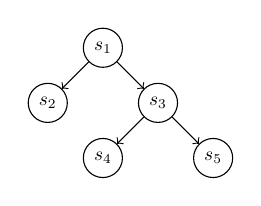
\begin{tikzpicture}[scale=0.7, every node/.style={transform shape}]
    \node[shape=circle,draw=black] (A) at (1,2) {$s_1$};
    \node[shape=circle,draw=black] (B) at (0,1) {$s_2$};
    \node[shape=circle,draw=black] (C) at (2,1) {$s_3$};
    \node[shape=circle,draw=black] (D) at (1,0) {$s_4$};
    \node[shape=circle,draw=black] (E) at (3,0) {$s_5$} ;
    \path [->] (A) edge node[left] {} (B);
    \path [->](A) edge node[left] {} (C);
    \path [->](C) edge node[left] {} (D);
    \path [->](C) edge node[left] {} (E);
\end{tikzpicture}
&\;\;\;\;&
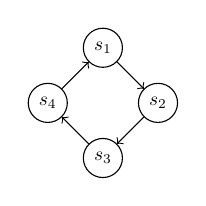
\begin{tikzpicture}[scale=0.7, every node/.style={transform shape}]
    \node[shape=circle,draw=black] (A) at (1,2) {$s_1$};
    \node[shape=circle,draw=black] (B) at (2,1) {$s_2$};
    \node[shape=circle,draw=black] (C) at (1,0) {$s_3$};
    \node[shape=circle,draw=black] (D) at (0,1) {$s_4$};
    \path [->] (A) edge node[left] {} (B);
    \path [->](B) edge node[left] {} (C);
    \path [->](C) edge node[left] {} (D);
    \path [->](D) edge node[left] {} (A);
\end{tikzpicture}
\end{tabular}
\end{center}

Dans la suite, on ne considère que des graphes acycliques.

\item Montrer que tout graphe acyclique admet un puits, c'est-à-dire un sommet sans successeur.  

Dans le cas général, le noyau d’un graphe $G=(S,A)$ est souvent difficile à calculer. Si la dimension du jeu n’est pas trop importante, on peut toutefois le faire en utilisant l'algorithme suivant : 
 \begin{center}
 \begin{minipage}{95mm}
  \begin{pcode-env}
  $N = \emptyset$ \;
  \While{il reste des sommets à traiter}
  {
  Chercher un sommet $s\in S$ sans successeur \;
  $N = N\bigcup \{s\}$ \;
  Supprimer $s$ de $G$ ainsi que ses prédécesseurs \;
  }
  \end{pcode-env}
\end{minipage}
\end{center}
\item Justifier que cet algorithme termine et renvoie un noyau.
\item Démontrer que ce noyau est unique. Conclure que le graphe du jeu de Chomp possède un unique noyau $N$. 
\item Appliquer cet algorithme pour calculer le noyau du jeu de Chomp à 2 lignes et 3 colonnes. Que peut-on dire du sommet (1,1) pour le joueur qui doit jouer ? En déduire à quoi correspondent les éléments du noyau.
\item Montrer que, dans le cas d'un graphe acyclique, tout joueur dont la position initiale n’est pas dans le noyau a une stratégie gagnante. Le joueur $J_1$ a-t-il une stratégie gagnante pour ce jeu dans le cas $l=2$ et $c=3$ ?
\end{enumerate}

\medskip
\textbf{Utilisation des attracteurs}

On modélise le jeu par un graphe biparti : pour ce faire, on dédouble les sommets du graphe précédent : un sommet $s_i$ génère donc deux sommets $s_i^1$ et $s_i^2$, $s_i^j$ étant le sommet $i$ contrôlé par le joueur $J_j$. On forme alors deux ensembles de sommets $S_1 = \{s_i^1\}_i$ et $S_2 = \{s_i^2\}_i$, et on construit le graphe de jeu orienté $G=(S,A)$ avec $S=S_1\bigcup S_2$ et $S_1\bigcap S_2=\emptyset$. De plus, $(s_i^1,s_j^2)\in A$ si le joueur 1 peut, par son choix de jeu, faire passer la tablette de l'état $s_i^1$ à l'état $s_j^2$. On raisonne de même pour $(s_i^2,s_j^1)\in A$.\\ 
On rappelle la définition d'un attracteur : soit $F_1$ l’ensemble des positions finales gagnantes pour $J_1$. On définit alors la suite d'ensembles $(\mathcal A_i)_{i\in\mathbb{N}}$ par récurrence : $\mathcal A_0=F_1$ et 
$$(\forall i\in\mathbb{N})\; \mathcal A_{i+1} = \mathcal A_i\cup\{s\in S_1/ \exists t\in \mathcal A_i, (s,t)\in A\}\cup \{s\in S_2\textrm{ non terminal}, \forall t\in S, (s,t)\in A \Rightarrow t\in \mathcal A_i\}$$
et  $\mathcal A = \displaystyle\bigcup_{i=0}^\infty \mathcal A_i$ est l'attracteur pour $J_1$.
\begin{enumerate}[resume]
\item Que représente l'ensemble $\mathcal A_{i}$ ?
\item Dans le cas du jeu de Chomp à deux lignes et trois colonnes (question 1), calculer les ensembles $\mathcal A_i$. Le joueur $J_1$ a-t-il une stratégie gagnante ? Comment le savoir à partir de $\mathcal A$ ?
\end{enumerate}

\paragraph*{Proposition de corrigé}

\begin{enumerate}
\item On obtient le graphe suivant (plus lisible avec des tablettes) : 
\begin{center}
  \begin{tikzpicture}[>=latex, node distance = 1cm]
    \node[] (0) {$(2,3)$};
    \node[] (1) [right = of 0] {$(2,1)$};
    \node[] (2) [above = of 1] {$(2,2)$};
    \node[] (3) [below = of 1] {$(1,3)$};
    \node[] (4) [right = of 1] {$(1,2)$};
    \node[] (5) [below = of 4] {$(1,1)$};
    \path[-latex]
    (0) edge (1)
    (0) edge (2)
    (0) edge (3)
    (1) edge (5)
    (2) edge (1)
    (2) edge (4)
    (3) edge (4)
    (3) edge (5)
    (4) edge (5)
    ;
  \end{tikzpicture}
\end{center}

\item Pour le premier graphe, le noyau est $(s_2,s_4,s_5)$. Pour le second il y a deux noyaux $(s_1,s_3)$ et $(s_2,s_4)$.
\item Soit $G$ un graphe acyclique sans puits. Soit $(s_0\cdots s_k)$ un chemin dans $G$. Comme $s_k$ n'est pas un puits, il existe un arc $(x_k,y)$ qui prolonge le chemin précédent. Il y a donc un chemin de longueur arbitraire dans $G$. Par le principe des tiroirs, tout chemin assez long contient nécessairement deux sommets qui coïncident, on a donc un cycle, en contradiction avec $G$ acyclique. Donc il existe au moins un puits dans $G$.
\item Supprimer des sommets d'un graphe acyclique le laisse acyclique donc la question 3 assure qu'on trouvera toujours un sommet $s$ convenable en ligne 3. Par conséquent, le nombre de sommets dans $G$ décroît strictement à chaque itération ce qui assure la terminaison de l'algorithme.

Par ailleurs, un sommet sans successeur doit être dans un noyau à cause de la deuxième propriété et donc tous ses prédécesseurs doivent être en dehors à cause de la première. Ces deux contraintes nécessaires sont garanties par l'algorithme. Elles sont suffisantes dans le cadre d'un graphe acyclique car tout sommet qui devrait nécessairement être dans un noyau et nécessairement ne pas y être ferait partie d'un cycle.
\item Travaillons par récurrence forte sur le nombre $n$ de sommets de $G$. Si $n=1$ ce seul sommet (puits) constitue le noyau. 

Sinon, soit $s$ un puits de $G$ (qui existe d'après la question 3). Ce sommet fait nécessairement partie de tous les noyaux de $G$. On note $P(s)$ l'ensemble des prédécesseurs de $s$. Le graphe $G$ privé de $s$ et des sommets de $P(s)$ reste acyclique et donc, par hypothèse de récurrence, a un noyau unique $N$. L'ensemble $N\bigcup\{s\}$ est un noyau de $G$ et par unicité de $N$ et nécessité du fait que $s$ soit dans tout noyau, c'est le seul.

\item Les sommets (2,2) et (1,1) constituent le noyau. La position (1,1) est perdante pour le joueur qui doit jouer (il mange le chocolat empoisonné), les éléments du noyau sont les sommets perdants et les autres sommets les positions gagnantes.
\item On montre qu’un joueur qui peut choisir $s_1$ dans le noyau ne peut pas perdre. Si $s_1$ n’a pas de successeur, l’adversaire ne peut plus jouer, il a perdu. Sinon, l’adversaire va choisir $s_2$ dans les successeurs de $s_1$. On a donc $s_2\in S\setminus N$ donc $s_2$ admet au moins un successeur dans $N$.
\item $\mathcal A_{i}$ est l'ensemble des sommets de $S$ à partir desquels $J_1$ peut forcer la partie à arriver en $F_1$ en moins de $i$ coups. 
\item $\mathcal A_0 = \{S_6^2\}, \mathcal A_1 = \{S_6^2,S_2^1,S_4^1\}=\mathcal A$. L'attracteur contient  exactement toutes les positions gagnantes pour $J_1$.
\end{enumerate}

\newpage
\section*{Exercices de type B}


\exocommand{\texttt{HORNSAT} (type B)}

\preambuleocaml \textit{On attend un style de programmation fonctionnel. L'utilisation des fonctions du module \mio{List} est autorisée ; celle des fonctions du module \mio{Option} est interdite.}

Une formule du calcul propositionnel est une \textit{formule de Horn} s'il s'agit d'une formule sous forme normale conjonctive (FNC) dans laquelle chaque clause (éventuellement vide, auquel cas la clause en question est la disjonction d'un ensemble vide de littéraux et est donc sémantiquement équivalente à $\bot$) contient au plus un littéral positif. Dans la suite, on considère qu'une clause d'une telle formule contient au plus une occurrence de chaque variable (en particulier, les clauses sont sans doublons).

\begin{enumerate}
    \item Les formules suivantes sont-elles des formules de Horn ? \begin{enumerate}[a)]
        \item $F_1 = (\neg x_0 \lor \neg x_1 \lor \neg x_3) \wedge (x_0 \lor \neg x_1) \wedge (\neg x_2 \lor x_0 \lor \neg x_3) \wedge (\neg x_0 \lor \neg x_3 \lor x_2) \wedge x_2 \wedge (\neg x_3 \lor \neg x_2)$.
        \item $F_2 = (x_0 \lor \neg x_1) \wedge (\neg x_2 \lor \neg x_3 \lor \neg x_0) \wedge \neg x_1 \wedge (x_1 \lor \neg x_1 \lor x_0) \wedge (\neg x_0 \lor x_2)$.
        \item $F_3 = (\neg x_1 \lor \neg x_4) \wedge x_1 \wedge (\neg x_0 \lor \neg x_3 \lor \neg x_4) \wedge (x_0 \lor \neg x_1) \wedge (x_2 \lor \neg x_3 \lor \neg x_4) \wedge (x_4 \lor \neg x_0 \lor \neg x_1)$.
    \end{enumerate}
\end{enumerate}

On utilise le type suivant pour manipuler les formules de Horn : une formule de Horn est une liste de clauses de Horn ; une clause étant la donnée d'un \mio{int option} valant \mio{None} si la clause ne contient pas de littéral positif et \mio{Some i} si $x_i$ en est l'unique littéral positif et d'une liste d'entiers correspondants aux numéros des variables intervenant dans les littéraux négatifs.

\begin{ocode}
   type clause_horn = int option * int list
   type formule_horn = clause_horn list
\end{ocode}

\begin{enumerate}[resume]
  \item \'Ecrire une fonction \mio{avoir_clause_vide : formule_horn -> bool} qui renvoie \mio{true} si et seulement si la formule en entrée contient une clause vide (donc ne contenant ni littéral positif, ni aucun littéral négatif).
\end{enumerate}
        

On appelle \textit{clause unitaire} une clause réduite à un littéral positif. Par ailleurs, \textit{propager} une variable $x_i$ dans une formule $F$ sous FNC consiste à modifier $F$ comme suit : \begin{itemize}
    \item Toute clause de $F$ qui ne fait pas intervenir la variable $x_i$ est conservée telle quelle.
    \item Toute clause de $F$ qui fait intervenir le littéral $x_i$ est supprimée entièrement.
    \item On supprime le littéral $\neg x_i$ de toutes les clauses de $F$ qui font intervenir ce littéral.
\end{itemize}

On souligne que supprimer $\neg x$ d'une clause $C$ qui ne fait intervenir que ce littéral ne revient pas à supprimer la clause $C$. On s'intéresse à l'algorithme $\mathcal{A}$ suivant dont on admet (pour le moment) qu'il permet de déterminer si une formule de Horn $F$ est satisfiable : \begin{center}
\begin{minipage}{11cm}
  \begin{pcode-nl-env}
    \While{il y a une clause unitaire $x_i$ dans $F$}
    {
      $F \leftarrow$ propager $x_i$ dans $F$ \;
    }
    \If{$F$ contient une clause vide}
    {
      \Return{faux} \;
    }
    \Else
    {
      \Return{vrai} \;
    } 
  \end{pcode-nl-env}  
\end{minipage}
\end{center}

\begin{enumerate}[resume]
    \item \`A l'aide de cet algorithme déterminer si les formules de Horn de la question 1 sont satisfiables. On utilisera ces formules pour tester les fonctions implémentées aux questions suivantes.
    \item \'{E}crire une fonction \mio{trouver_clause_unitaire : formule_horn -> int option} renvoyant \mio{None} si la formule en entrée n'a pas de clause unitaire et \mio{Some i} où $x_i$ est l'une des clauses unitaires sinon.
    \item Justifier que propager une variable dans une formule de Horn donne une formule de Horn. \'{E}crire une fonction \mio{propager : formule_horn -> int -> formule_horn} qui prend en entrée une formule de Horn $F$ et un entier $i$ et calcule la formule résultat de la propagation de $x_i$ dans~$F$.
    \item Déduire des questions précédentes une fonction \mio{etre_satisfiable : formule_horn -> bool} renvoyant \mio{true} si et seulement si la formule de Horn en entrée est satisfiable.
    \item Quelle est la complexité de votre algorithme en fonction de la taille de la formule en entrée ? Que peut-on dire des problèmes de décision \texttt{SAT} et \texttt{HORN-SAT} (dont la définition est la même que celle de \texttt{SAT} à ceci près que les formules considérées sont supposées être des formules de Horn) ?
    \item On s'intéresse à présent à la correction de l'algorithme $\mathcal{A}$. \begin{enumerate}[a)]
    \item Si $F$ est une clause de Horn sans clause unitaire ni clause vide, donner une valuation simple qui satisfait $F$.
        \item On admet que si $F$ est une formule de Horn faisant intervenir une clause unitaire $x_i$ et $F'$ est le résultat de la propagation de $x_i$ dans $F$, alors que $F$ est satisfiable si et seulement si $F'$ est satisfiable. En déduire la correction de l'algorithme $\mathcal{A}$.
    \end{enumerate}
    \item Expliquer comment on pourrait modifier les fonctions précédentes afin de déterminer une valuation satisfaisant une formule de Horn dans le cas où elle existe plutôt que de juste dire si elle est satisfiable ou non. On ne demande pas d'implémentation.
\end{enumerate}


\paragraph*{Proposition de corrigé}

  \begin{enumerate}
      \item $F_1$ et $F_3$ sont des formules de Horn mais pas $F_2$, ce qui est implicitement suggéré par le code.
  \item Avec notre modélisation, la clause vide est \mio{(None, [])} d'où :
  \begin{ocode}
    let avoir_clause_vide (f:formule_horn) :bool = 
      List.mem (None, []) f
    \end{ocode}
  
  \item La formule $F_1$ est satisfiable d'après cet algorithme mais pas $F_3$.
  
  Techniquement on peut arrêter les propagations dès qu'on produit une clause vide. 
  
  \item On propose : \begin{ocode}
let rec trouver_clause_unitaire (f:formule_horn) :int option = match f with
  |[] -> None
  |(Some v,l)::q -> if l = [] then Some v else trouver_clause_unitaire q
  |_::q -> trouver_clause_unitaire q
  \end{ocode}
    
  \item La fonction auxiliaire \mio{enlever_neg} supprime si elle existe la seule occurrence d'un entier dans une liste d'entiers (on utilise ici l'hypothèse selon laquelle il n'y a pas de littéral en doublon dans nos clauses de Horn) puis on applique le principe décrit par l'énoncé.
  
  \newpage
  
  \begin{ocode}
let rec propager (f:formule_horn) (v:int) :formule_horn =
  let rec enlever_neg (l:int list) :int list = match l with
    |[] -> []
    |t::q when t = v -> q
    |t::q -> t::(enlever_neg q)
  in
  match f with
  |[] -> []
  |(i,l)::q -> match i with
                 |Some t when t = v -> propager q v
                 |_ -> (i, enlever_neg l)::(propager q v)
  \end{ocode}
   

  La formule résultant d'une propagation dans une formule de Horn reste une formule de Horn : c'est toujours une FNC et on ne fait que supprimer des clauses / littéraux (donc s'il y avait au plus un littéral positif par clause, en supprimant des choses cette propriété est conservée).
  
  \item On applique l'algorithme donné par l'énoncé en imbriquant les fonctions précédentes : \begin{ocode}
let rec etre_satisfiable (f:formule_horn) :bool =
  match (trouver_clause_unitaire f) with
  |None -> not (avoir_clause_vide f)
  |Some v -> etre_satisfiable (propager f v)
\end{ocode}
    
  \item La fonction \mio{trouver_clause_unitaire} est linéaire en $n$ la taille de la formule en entrée. Une propagation se fait aussi linéairement en la taille de la formule dans laquelle on propage. Comme une propagation supprime au moins une clause de la formule (la clause unitaire responsable de la propagation), on fera au plus $m$ étapes de "recherche de clause unitaire + propagation" où $m$ est le nombre de clauses.
  
  De plus, la recherche d'une clause vide dans une formule se fait linéairement en le nombre de clauses. On aboutit donc grossièrement (c'est-à-dire sans compter qu'au fil des propagations la taille de la formule réduit - de toutes façons ça ne changerait probablement pas grand chose) à une complexité pour \mio{etre_satisfiable} en $O(mn + m) = O(n^2)$.
  
  On en déduit que \texttt{HORN-SAT} $\in$ P alors qu'on sait que \texttt{SAT} est NP-complet. Sous réserve que P $\neq$ NP, étudier la satifiabilité de formules de Horn est donc un problème bien plus facile que lorsqu'il n'y a pas d'hypothèse sur les formules.
  
  \item \begin{enumerate}[a)]
      \item La valuation qui assigne faux à toutes les variables convient. En effet, s'il n'y a ni clause unitaire ni clause vide, toutes les clauses contiennent au moins une variable niée.
      \item Si $F$ est une formule de Horn, notons $\Pi(F)$ la formule de Horn obtenue après toutes les propragations successives de la boucle tant que dans l'algorithme $\mathcal{A}$. La propriété de l'énoncé permet de montrer par récurrence que $F$ et $\Pi(F)$ sont équisatisfiables.
      
      Or $\Pi(F)$ est satisfiable si et seulement si cette formule de Horn ne contient pas la clause vide : le sens direct est immédiat puisque une FNC contenant une clause vide n'est jamais satisfiable (cette clause ne l'étant pas) ; le sens réciproque est fourni par la question 7a.      

  \end{enumerate}
      \item Le principe est de garder trace des variables que l'on propage : on les assigne toutes à vrai. Toutes les variables non propagées sont quant à elles assignées à faux.
  
  
  \end{enumerate}

  \newpage

  \exocommand{Mots de Dyck (type B)}


\preambulec

\textit{La compilation du code compagnon initial avec \mib{make safe} provoque des warnings attendus qui seront résolus lors de l'implémentation des fonctions demandées par le sujet.}

On s'intéresse dans cet exercice aux mots de Dyck, c'est-à-dire aux mots bien parenthésés.
Dans ce type de mots, toute parenthèse ouverte "(" est fermée ")" et 
une parenthèse ne peut être fermée si elle ne correspond pas à une parenthèse préalablement ouverte.

Par exemple pour deux couples de parenthèses, "(())" et "()()" sont des chaînes de parenthèses bien formées. 
"())(" et ")()(" ne le sont pas.

On admet que le nombre de mots bien parenthésés à $n$ couples de parenthèses est donné par les nombres de Catalan définis par la formule suivante :
$$C_n = \frac{(2n)!}{(n+1)!n!} \text{ pour } n\geq 0$$

On rappelle que le type \texttt{uint64\_t} est un type entier non signé codé sur 64 bits.

\begin{enumerate}
\item Complétez dans le code compagnon la fonction dont le prototype est \texttt{uint64\_t catalan(int n)}.
Vous pouvez utiliser une fonction auxiliaire si cela vous semble pertinent.
\item Que va-t-il se passer si on tente d’afficher \texttt{catalan(n)} pour \texttt{n} un peu grand ? Le constatez-vous ici ?
\end{enumerate}

On cherche maintenant à afficher le nombre de mots (chaînes) bien parenthésés avec $n$ fixé couples de parenthèses, ainsi que les mots eux-mêmes.

Un algorithme de force brute pour déterminer toutes les chaînes à $n$ couples de parenthèses bien formées 
consiste à générer toutes les possibilités puis à ne garder que les chaînes bien formées.

\begin{enumerate}
\addtocounter{enumi}{2}
\item Complétez dans le code compagnon la fonction dont le prototype est \texttt{bool verification(char * mot)}. Cette fonction renvoie \texttt{true} si le mot fourni en paramètre $\texttt{mot}$ est bien parenthésé, \texttt{false} sinon.
\item Quelle est la complexité de cette vérification ?
\item Quelle est la complexité finale de l'algorithme de force brute ?
\end{enumerate}

On appelle \texttt{n} le nombre de couples de parenthèses voulu.
Dans le fichier compagnon fourni, le nombre de couples a été limité à 18.

On vous propose de coder l'énumération des chaînes de parenthèses bien formées en appliquant l'algorithme de backtracking suivant, dont on admet qu'il est correct :
on compte le nombre de parenthèses ouvertes \texttt{o} et le nombre de parenthèses fermées \texttt{f} dans une chaîne de caractères courante (vide au départ).

\begin{itemize}
\item Si $\texttt{o = f = n}$, on a trouvé une chaîne bien formée. 
\item Si $\texttt{o < n}$, on ajoute une parenthèse ouvrante et on relance.
\item Si $\texttt{f < o}$, on ajoute une parenthèse fermante et on relance.
\end{itemize}

Cet algorithme est à implémenter dans la fonction dont le prototype est \texttt{void dyck(char s[N], int o, int f, int n)}
 qui affiche sur la sortie standard les chaînes de parenthèses bien formées avec \texttt{n} couples de parenthèses lorsque \texttt{s}
est la chaîne de caractère courante, \texttt{o} est son nombre de parenthèses ouvrantes et \texttt{f} est son nombre de parenthèses fermantes.

\begin{enumerate}
\addtocounter{enumi}{5}
\item Compléter la fonction \texttt{dyck} pour afficher les chaînes bien parenthésées avec 5 couples de parenthèses.
\item Adapter la fonction \texttt{dyck} pour calculer le nombre de mots obtenus. Combien de mots trouvez-vous pour 16 couples de parenthèses ?
\item Adapter la fonction \texttt{dyck} pour stocker les mots bien parenthésés dans une liste chaînée et les afficher après l'appel à la fonction. Vous trouverez dans le code compagnon une structure 
qui peut vous aider.
\end{enumerate}

\paragraph*{Proposition de corrigé}

\begin{enumerate}
\item Une solution et d'implémenter une factorielle. On peut aussi simplifier la formule donnée (ce qui permet de repousser un peu plus loin le dépassement).
\begin{ccode}
uint64_t fact(int n) {
    uint64_t r = 1;
    for(int i = 2; i <= n; i = i + 1){
        r = r * i;
    }
    return r;
}

uint64_t catalan1(int n) {
    return fact(2*n)/fact(n+1)/fact(n);
}\end{ccode}
  \item On obtient un dépassement d'entier.
        Expérimentalement, si on utilise la fonction factorielle, le résultat devient faux pour $n=11$.
        En simplifiant la formule en $2n \times ... \times (n+2)/n!$, c'est pour $n=16$ que ça coince.
        Dans tous les cas, le dépassement finira par arriver provoquant un comportement indéfini.
\item On utilise un compteur qui indique le nombre de parenthèses ouvertes : on l'incrémente lorsqu'on rencontre une parenthèse ouvrante et on le décrémente lorsqu'on rencontre une parenthèse fermante. Si ce compteur devient négatif, le mot n'est pas bien parenthésé puisqu'il y a trop de parenthèses fermantes et on peut donc interrompre l'exécution (même si on peut se passer de cette subtilité). En fin de décompte, le compteur devrait être nul si le mot est bien parenthésé.
\begin{ccode}
bool verification(char * mot) {
    int i = 0;
    bool fin = false;
    int compteur = 0;
    bool resultat = false;
    while (!fin && (mot[i] != '\0')) {
        if (mot[i]=='(') {
            compteur++;
        }
        else if (mot[i] == ')') {
            compteur = compteur - 1;
        }
        if (compteur<0) {
            fin = true;
        }
        i = i + 1;
    }
    if (compteur == 0) {
        resultat = true;
    }
    return resultat;
}
\end{ccode}
\item On obtient un algorithme linéaire en la taille du mot en entrée.
\item Il y a $4^n$ mots à générer (puisqu'un mot à $n$ couples de parenthèses possède $2n$ lettres). Pour chacun, la vérification de s'il est bien formé se fait en $O(2n) = O(n)$. \`A supposer que la construction des mots ne soit pas coûteuse, on obtient une complexité pour l'algorithme naïf en $O(4^n \times n)$.
\item Voici une proposition qui répond aux questions 6, 7 et 8.

\begin{ccode}
  void dyck(char s[N], int o, int f, int n, uint64_t* r,
            struct liste_s ** liste) {
    if (f == n) {
        if (liste != NULL) {
            struct liste_s * c = malloc(sizeof(struct liste_s));
            strcpy(c->chaine, s);
            c->suivant = *liste;
            *liste = c;
        }
        else {
            printf("%s\n", s);
        }
        (*r) = (*r) + 1;
        return;
    }
    if (o<n) {
        // printf("on ajoute (\n");
        char res[N];
        strcpy(res, s);
        strcat(res, "(");
        dyck(res, o+1, f, n, r, liste);
    }
    if (f<o) {
        // printf("on ajoute )\n");
        char res[N];
        strcpy(res, s);
        strcat(res, ")");
        dyck(res, o, f+1, n, r, liste);
    }
  }
\end{ccode}

\item Une façon de faire est d'ajouter un paramètre passé par pointeur pour compter ce nombre. On pourrait aussi utiliser une variable globale. On trouve $35357670$ mots corrects pour $n = 16$.
\item Voir la proposition en question 6.
\end{enumerate}
\end{document}
